% Reset dei contatori per l'appendice
\setcounter{figure}{0}
\renewcommand{\thefigure}{A.\arabic{figure}}
\setcounter{table}{0}
\renewcommand{\thetable}{A.\arabic{table}}

\section{Feature Engineering e Riduzione della Dimensionalità}
\label{app:feature_engineering}

Questa sezione documenta le trasformazioni applicate allo spazio delle feature originali al fine di migliorarne la qualità informativa e la trattabilità computazionale. L'attenzione si è focalizzata sulla gestione delle variabili categoriche ad alta cardinalità che presentano sfide critiche legate alla sparsità e alla stabilità statistica delle stime.

\subsection{Gestione della Cardinalità: Il caso \texttt{native.country}}

L'analisi preliminare della variabile \texttt{native.country} ha evidenziato una distribuzione altamente sbilanciata e frammentata. La variabile originale presentava numerosi livelli (paesi) con frequenze assolute trascurabili ($n_i < 50$), configurando un problema di \textit{Sparse Classes}.

Mantenere tale granularità comporterebbe due rischi principali in fase di modellazione:
\begin{enumerate}
    \item \textbf{Esposizione alla "Curse of Dimensionality":} L'applicazione di tecniche di codifica come il One-Hot Encoding genererebbe una matrice sparsa con dozzine di colonne quasi vuote.
    \item \textbf{Instabilità dell'Inferenza:} I coefficienti stimati per le categorie rare sarebbero caratterizzati da varianza elevata e scarsa generalizzabilità (rischio di overfitting su specifici pattern di rumore).
\end{enumerate}

\subsection{Strategia di Aggregazione (Binning)}
Per mitigare tali criticità, è stata implementata una strategia di riduzione della dimensionalità basata sull'aggregazione semantica. La variabile è stata trasformata in una feature binaria \texttt{native\_region} secondo la seguente logica di mappatura $f(x)$:

\begin{equation}
    f(x) = 
    \begin{cases} 
    \text{'USA'} & \text{se } x = \text{'United-States'} \\
    \text{'Other'} & \text{altrimenti}
    \end{cases}
\end{equation}

\noindent
Tale trasformazione assume che la distinzione discriminante principale nel dataset (Census Income, di natura socio-economica statunitense) risieda nella dicotomia tra nativi e non nativi, piuttosto che nelle specificità del singolo paese di origine estero.

\subsection{Analisi della Distribuzione Post-Processing}

A seguito della trasformazione, è stata condotta un'analisi della frequenza per valutare il nuovo assetto distributivo della feature \texttt{native\_region}.

\begin{figure}[H]
    \centering
    % Placeholder per l'immagine generata dal codice Python
    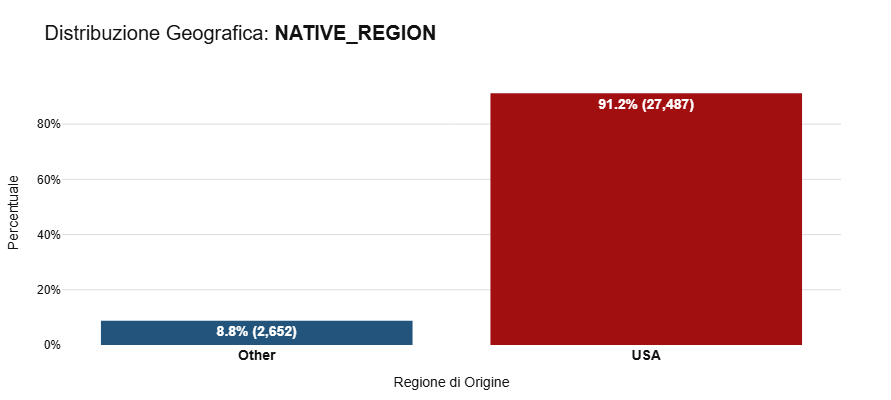
\includegraphics[width=1\textwidth]{figures/bilanciamento_country.png} 
    \caption{Distribuzione delle frequenze per la feature ingegnerizzata \texttt{native\_region}. Si evidenzia la netta predominanza della classe 'USA'.}
    \label{fig:bilanciamento_country.png}
\end{figure}

\noindent
L'analisi quantitativa (Figura \ref{fig:bilanciamento_country.png}) evidenzia che la categoria 'USA' assorbe la vasta maggioranza delle osservazioni ($>90\%$). Sebbene l'operazione abbia risolto il problema della sparsità, ha introdotto (o meglio, cristallizzato) un forte sbilanciamento di classe.

\subsection{Implicazioni per la Modellazione}
La concentrazione di massa sulla classe 'USA' riduce la varianza della feature, limitandone potenzialmente il potere predittivo (\textit{Information Gain}). Una variabile con una categoria dominante al $90\%+$ tende ad approssimarsi a una costante.
Tuttavia, il mantenimento della distinzione 'USA' vs 'Other' è ritenuto preferibile alla rimozione totale della variabile, in quanto permette al modello di catturare eventuali bias sistemici legati allo status di immigrazione, pur in un contesto di bassa entropia.

\newpage